\documentclass{article}
\usepackage[utf8]{inputenc}
\usepackage[margin=1in]{geometry}
\usepackage{graphicx}
\usepackage{float}

\title{LatexIt}
\author{Auto-translator built by SHASHVAT SRIVASTAVA}
\date{November 2019}

\begin{document}
\maketitle
\tableofcontents\newpage 
 \section{2012}9/5\\
Lecture I
\begin{itemize}
\item  professor has a math PhD???
\item  other professor does chemistry ??? Wanted to study drama too
\end{itemize}
Important central idea of this class: unifying\\
principles.\\
Not facts\\
only!\\
Important stuff
\begin{itemize}
\item  Read the course website.
\end{itemize}
I - Course policies, recitation sections, etc.
\begin{itemize}
\item  Office hours, recitations start next week
\item  Fill out the mock submission survey!
\end{itemize}
\begin{itemize}
\item  MITX?
\end{itemize}
\begin{itemize}
\item 4 exams + final. (This is a change!) Also you can drop an exam.
You Do need to show up.
\end{itemize}
\begin{itemize}
\item  Problem sets cannot be late. Collaboration is fine, but not copying.
\item  Different styles of learning
\begin{itemize}
\item  Paper textbook (Life), series of videos (see MITX), online textbook (!)
\item  Choose what you want for your own learning
\end{itemize}
\end{itemize}
What is this class?
\begin{itemize}
\item  Medicine rapidly developing in the present
\end{itemize}
\begin{itemize}
\item  Cancer therapy, etc.
DNA fingerprinting - then privacy issues, ancestry, etc.
\item  Constantly changing \& driving forward? Things like genome editing!
"Diversity of life" - what's the common operating system?
\end{itemize}
\begin{itemize}
\item  Different "levels" — biospheres, ecosystems, organisms, organs, tissues, cells,
organelles, molecules (big to small)
\begin{itemize}
\item  We focus on the small things because they are common.
\end{itemize}
\end{itemize}

                            \begin{figure}[H]
                            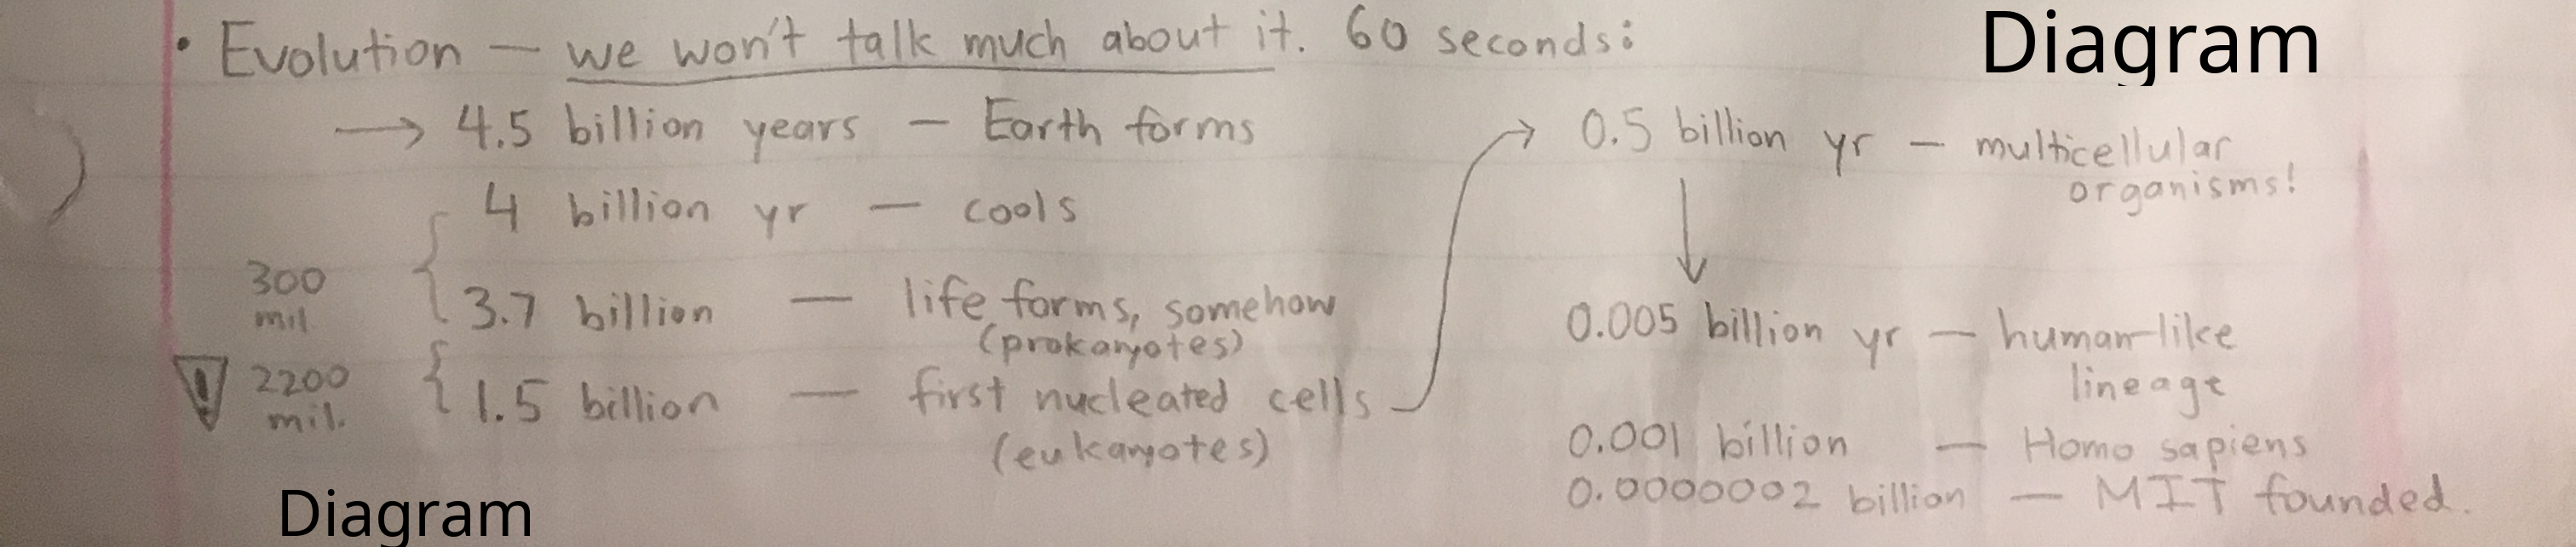
\includegraphics[width=0.9\textwidth]{q0q0.png}
                            \end{figure}
                            \newpage 
 \section{2012}9/5\\
Lecture I
\begin{itemize}
\item  professor has a math PhD???
\item  other professor does chemistry ??? Wanted to study drama too
\end{itemize}
Important central idea of this class: unifying\\
principles.\\
Not facts\\
only!\\
Important stuff
\begin{itemize}
\item  Read the course website.
\end{itemize}
I - Course policies, recitation sections, etc.
\begin{itemize}
\item  Office hours, recitations start next week
\item  Fill out the mock submission survey!
\end{itemize}
\begin{itemize}
\item  MITX?
\end{itemize}
\begin{itemize}
\item 4 exams + final. (This is a change!) Also you can drop an exam.
You Do need to show up.
\end{itemize}
\begin{itemize}
\item  Problem sets cannot be late. Collaboration is fine, but not copying.
\item  Different styles of learning
\begin{itemize}
\item  Paper textbook (Life), series of videos (see MITX), online textbook (!)
\item  Choose what you want for your own learning
\end{itemize}
\end{itemize}
What is this class?
\begin{itemize}
\item  Medicine rapidly developing in the present
\end{itemize}
\begin{itemize}
\item  Cancer therapy, etc.
DNA fingerprinting - then privacy issues, ancestry, etc.
\item  Constantly changing \& driving forward? Things like genome editing!
"Diversity of life" - what's the common operating system?
\end{itemize}
\begin{itemize}
\item  Different "levels" — biospheres, ecosystems, organisms, organs, tissues, cells,
organelles, molecules (big to small)
\begin{itemize}
\item  We focus on the small things because they are common.
\end{itemize}
\end{itemize}

                            \begin{figure}[H]
                            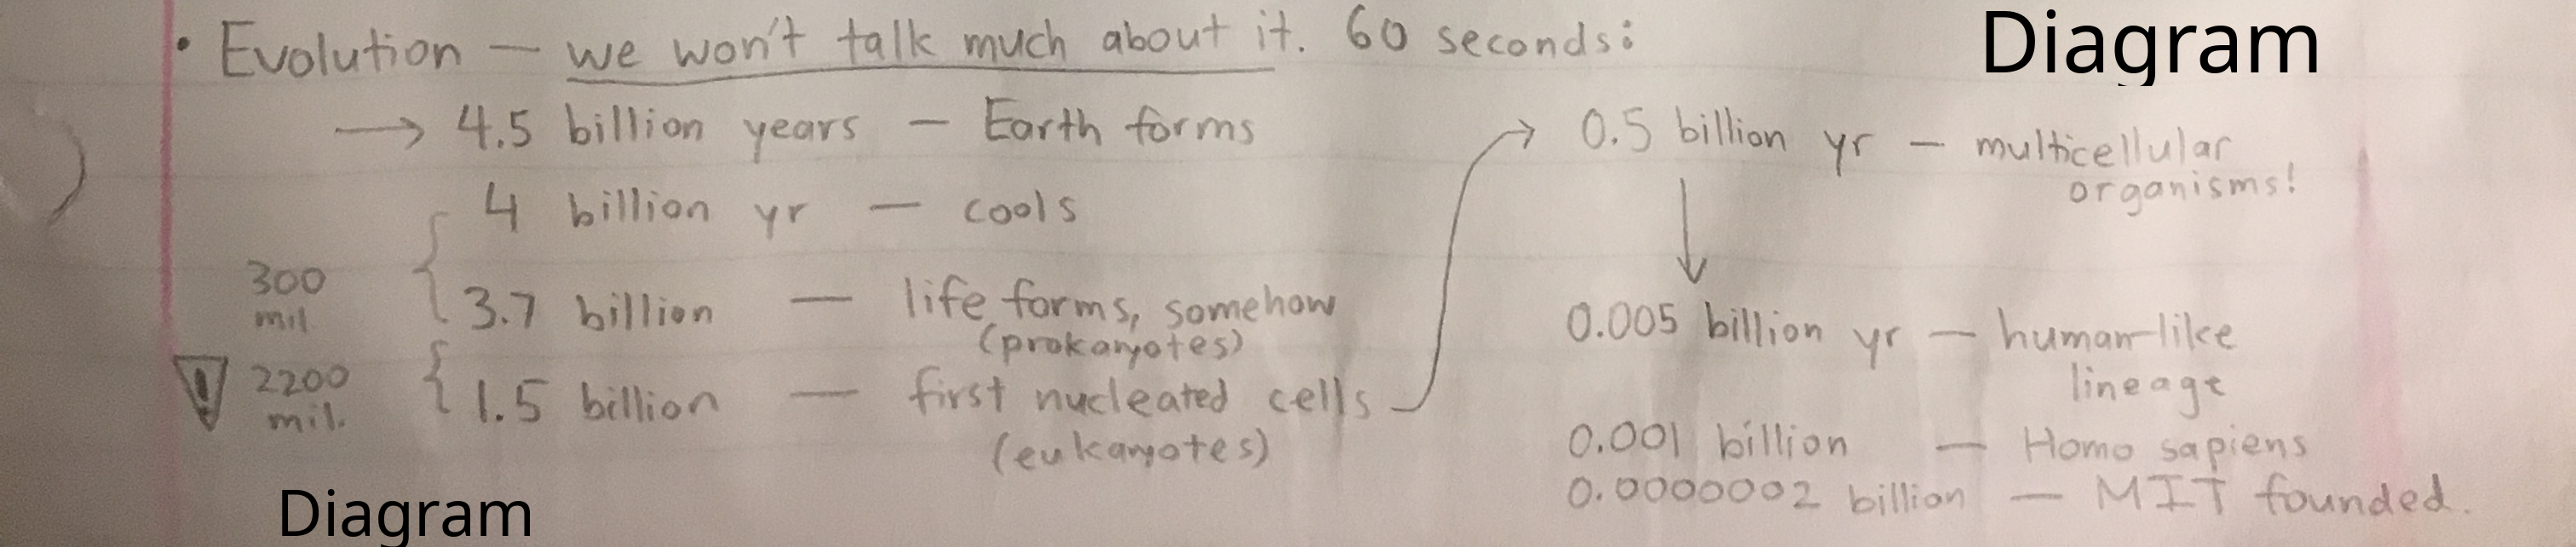
\includegraphics[width=0.9\textwidth]{q1q0.png}
                            \end{figure}
                            \newpage 
 \section{2012}9/5\\
Lecture I
\begin{itemize}
\item  professor has a math PhD???
\item  other professor does chemistry ??? Wanted to study drama too
\end{itemize}
Important central idea of this class: unifying\\
principles.\\
Not facts\\
only!\\
Important stuff
\begin{itemize}
\item  Read the course website.
\end{itemize}
I - Course policies, recitation sections, etc.
\begin{itemize}
\item  Office hours, recitations start next week
\item  Fill out the mock submission survey!
\end{itemize}
\begin{itemize}
\item  MITX?
\end{itemize}
\begin{itemize}
\item 4 exams + final. (This is a change!) Also you can drop an exam.
You Do need to show up.
\end{itemize}
\begin{itemize}
\item  Problem sets cannot be late. Collaboration is fine, but not copying.
\item  Different styles of learning
\begin{itemize}
\item  Paper textbook (Life), series of videos (see MITX), online textbook (!)
\item  Choose what you want for your own learning
\end{itemize}
\end{itemize}
What is this class?
\begin{itemize}
\item  Medicine rapidly developing in the present
\end{itemize}
\begin{itemize}
\item  Cancer therapy, etc.
DNA fingerprinting - then privacy issues, ancestry, etc.
\item  Constantly changing \& driving forward? Things like genome editing!
"Diversity of life" - what's the common operating system?
\end{itemize}
\begin{itemize}
\item  Different "levels" — biospheres, ecosystems, organisms, organs, tissues, cells,
organelles, molecules (big to small)
\begin{itemize}
\item  We focus on the small things because they are common.
\end{itemize}
\end{itemize}

                            \begin{figure}[H]
                            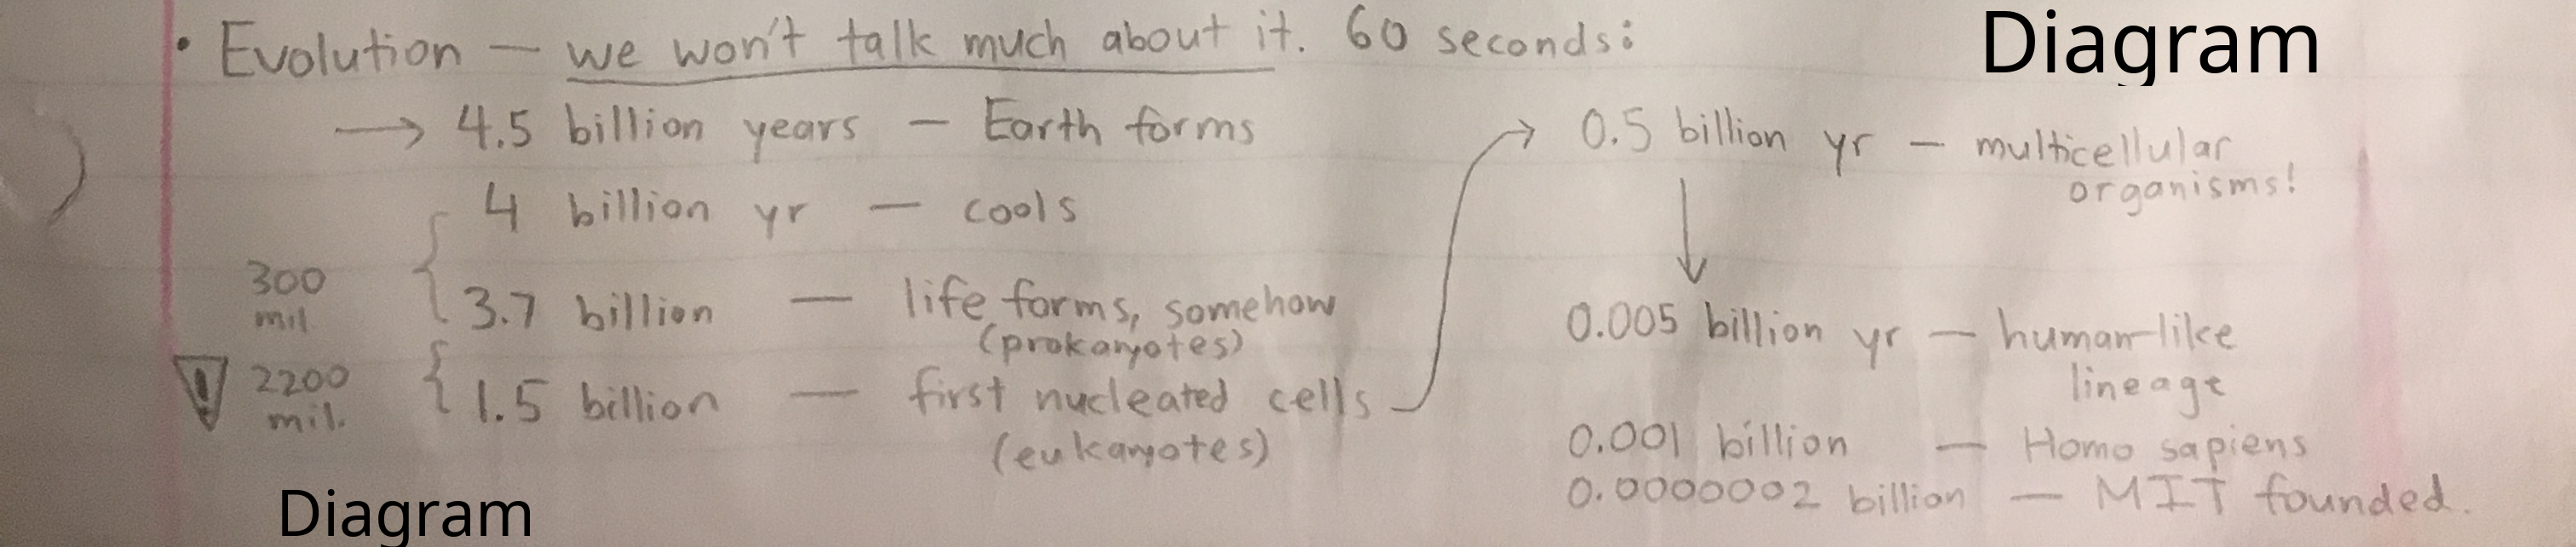
\includegraphics[width=0.9\textwidth]{q2q0.png}
                            \end{figure}
                            \newpage 
 \section{2012}9/5\\
Lecture I
\begin{itemize}
\item  professor has a math PhD???
\item  other professor does chemistry ??? Wanted to study drama too
\end{itemize}
Important central idea of this class: unifying\\
principles.\\
Not facts\\
only!\\
Important stuff
\begin{itemize}
\item  Read the course website.
\end{itemize}
I - Course policies, recitation sections, etc.
\begin{itemize}
\item  Office hours, recitations start next week
\item  Fill out the mock submission survey!
\end{itemize}
\begin{itemize}
\item  MITX?
\end{itemize}
\begin{itemize}
\item 4 exams + final. (This is a change!) Also you can drop an exam.
You Do need to show up.
\end{itemize}
\begin{itemize}
\item  Problem sets cannot be late. Collaboration is fine, but not copying.
\item  Different styles of learning
\begin{itemize}
\item  Paper textbook (Life), series of videos (see MITX), online textbook (!)
\item  Choose what you want for your own learning
\end{itemize}
\end{itemize}
What is this class?
\begin{itemize}
\item  Medicine rapidly developing in the present
\end{itemize}
\begin{itemize}
\item  Cancer therapy, etc.
DNA fingerprinting - then privacy issues, ancestry, etc.
\item  Constantly changing \& driving forward? Things like genome editing!
"Diversity of life" - what's the common operating system?
\end{itemize}
\begin{itemize}
\item  Different "levels" — biospheres, ecosystems, organisms, organs, tissues, cells,
organelles, molecules (big to small)
\begin{itemize}
\item  We focus on the small things because they are common.
\end{itemize}
\end{itemize}

                            \begin{figure}[H]
                            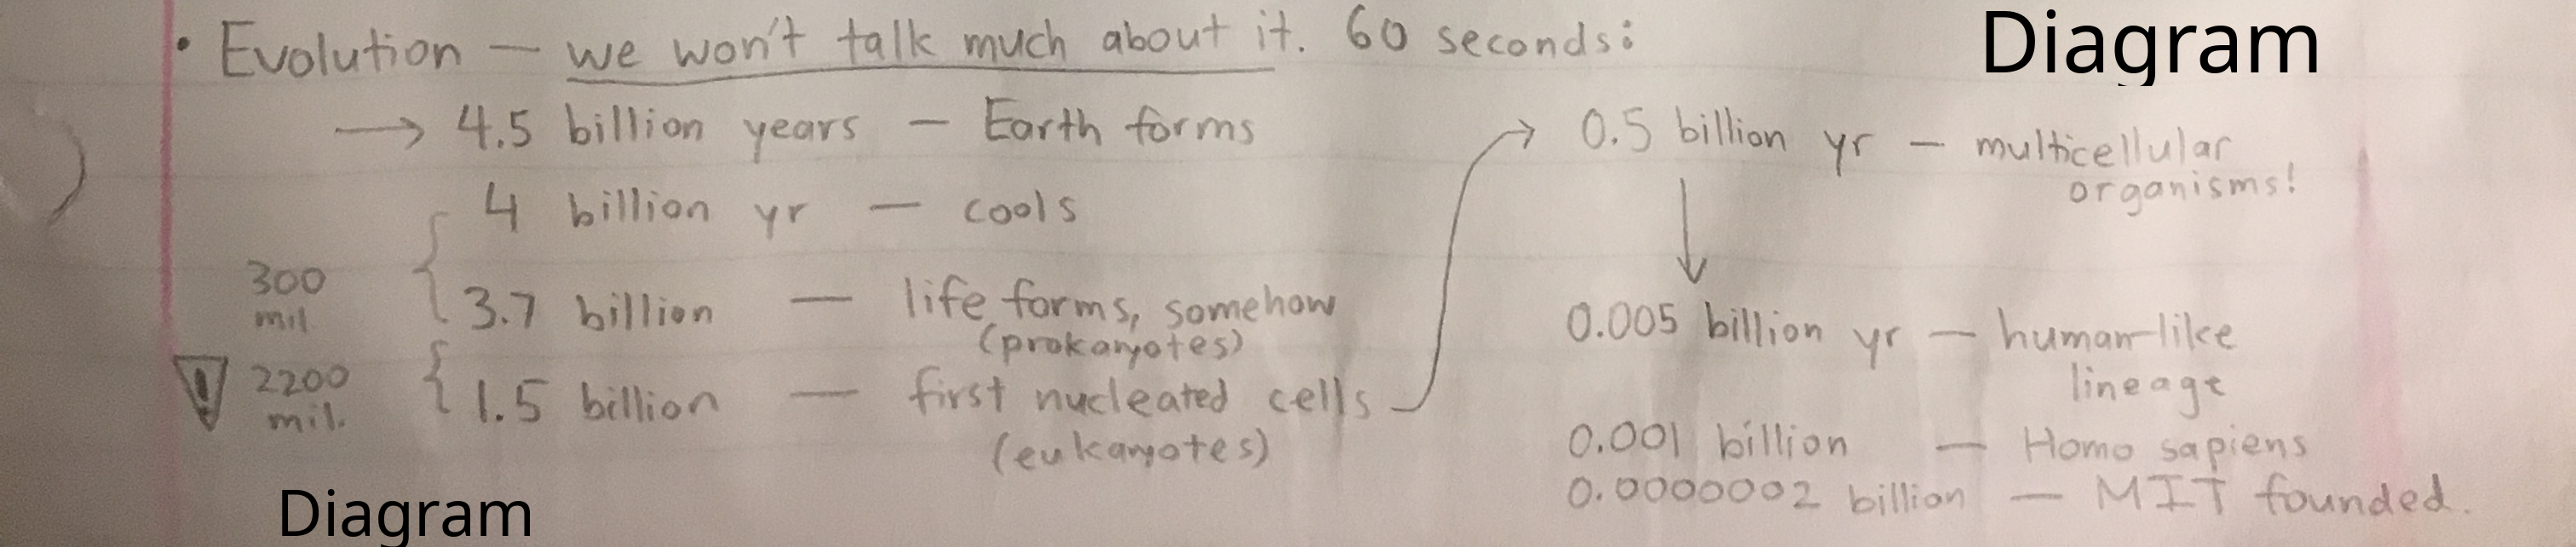
\includegraphics[width=0.9\textwidth]{q3q0.png}
                            \end{figure}
                            \end{document}